% ============================== CHAPTER 4 ==============================
\chapterdivider{4}{IMPLEMENTATION \& RESULTS}
\chapter{Implementation \& Results}

\section{Introduction}
This chapter describes how the methodology of Chapter~3 was turned into working software and what it produced. The implementation has four parts: the Python reference implementation of the protocol with its pluggable resolvers; the C port of the device side for the ESP8266; the measurement and simulation pipeline; and the ProVerif models. The results are evaluated in the same order as the objectives: conformance of the implementations to the independent vectors, correctness of the test suite, probe counts against their closed forms, session latency and storage in the network model, desynchronisation behaviour, and the formal security properties.

Unless stated otherwise, the numbers come from the data committed in the project repository (commit \texttt{e21993a}), which is the data used in the project's paper. For this report, the test suite, the C vector check, the interoperability check, the desynchronisation check, the probe-count sweep and the figure generation were re-run on the machine described in Table~\ref{tab:hw}; their logs are kept in the \texttt{results/} folder next to this report. The OMNeT++ sweep and the ProVerif models were not re-run for this report; their committed outputs are used.

\section{Implementation}
\subsection*{Python reference implementation}
The package \texttt{hybrid\_ecc\_auth} follows the layered architecture of Figure~\ref{fig:arch}. The \emph{crypto} layer instantiates the paper's primitives: $H_1$, $H_2$ and $H_3$ with SHA-256, the KDF with HKDF-SHA256, AEAD with AES-256-GCM, and 128-bit nonces from the operating system's secure generator. P-256 scalar multiplication is used only in the offline phase. The \emph{protocol} layer implements the trusted authority (\texttt{TrustedAuthority.enroll}), the device (\texttt{Device.build\_auth\_request}, \texttt{complete\_auth}) and the server (\texttt{Server.handle\_auth\_request}), with field names that follow the paper's notation so that each line can be traced to its equation. Messages are versioned and serialised as JSON with base64 fields; an $M_1$ is 216 bytes on the wire. Listing~\ref{lst:server} shows the server's handling of $M_1$: resolution comes first, then the block-list check, the AEAD decryption, and the check that the decrypted pseudonym and epoch match the header.

\par\noindent\begin{minipage}{\linewidth}
\begin{lstlisting}[language=Python, caption={Server handling of $M_1$ (\texttt{protocol/server.py}, abridged)}, label=lst:server]
def handle_auth_request(self, msg1_bytes: bytes) -> AuthResult:
    msg1 = Message1.from_bytes(msg1_bytes)
    peer_identity, epoch = self.resolve_pseudonym(msg1.pid)
    if self.session_log.is_blocked(peer_identity):        # fail fast
        raise BlockedEntity(...)
    k_star = self.get_pairwise_root(peer_identity)
    try:
        plaintext = aead.decrypt(k_star, msg1.gcm_nonce, msg1.ciphertext, msg1.tag)
    except InvalidTag as exc:
        self.session_log.record_failure(peer_identity)
        raise IntegrityError(...) from exc
    pid_in_plaintext, n_i = plaintext[:32], plaintext[32:-8]
    epoch_in_plaintext = int.from_bytes(plaintext[-8:], "big")
    if pid_in_plaintext != msg1.pid or epoch_in_plaintext != epoch:
        self.session_log.record_failure(peer_identity)
        raise IntegrityError(...)
    self.resolver.accept(peer_identity, epoch, n_i)
    self.session_log.record_success(peer_identity)
    n_j = generate_nonce(self.nonce_bits)
    session_key = derive_session_key(k_star, n_i, n_j, epoch)
    gcm_nonce2, ct2, tag2 = aead.encrypt(k_star, n_j + epoch.to_bytes(8, "big"),
                                         aad=msg1.pid + n_i)
    ...
\end{lstlisting}
\end{minipage}\par

The \emph{storage} layer's \texttt{SessionLog} keeps, per peer, the last accepted epoch and the search window $[\ell-L,\ell+F]$ with $L=16$ and $F=8$, rejects stale epochs as replays, and block-lists a peer after three failed attempts. The \emph{demo} layer adds length-prefixed TCP framing and the command-line tools \texttt{hea-ta}, \texttt{hea-server} and \texttt{hea-device}; the device tool can replay its last $M_1$ to demonstrate replay rejection.

\subsection*{Pluggable resolvers}
Every resolver implements the interface of Listing~\ref{lst:resolver}: \texttt{attach} is called once with the enrolled secrets, \texttt{resolve} for every $M_1$, and \texttt{accept} after $M_1$ has been verified. Every $H_2$ evaluation goes through one method, which counts it either as a probe (work for an incoming message) or as precomputation. Strategies O1--O4 and TM live in \texttt{protocol/resolution.py} and run inside the real handshake; CR and MW change $M_1$ and are implemented at the resolution level in \texttt{evaluation/resolution/rfid\_schemes.py}.

\par\noindent\begin{minipage}{\linewidth}
\begin{lstlisting}[language=Python, caption={Resolver interface and strategies O1 and O2 (\texttt{protocol/resolution.py}, abridged)}, label=lst:resolver]
class Resolver:
    def _h2(self, lam, epoch, *, precompute=False):
        if precompute: self.precompute_probes += 1
        else:          self.probes += 1
        return h2_pseudonym(lam, epoch)

class LinearScan(Resolver):                      # O1
    def resolve(self, pid):
        log = self.session_log
        for peer_identity, peer_lam in self.peer_secrets.items():
            for epoch in log.epoch_search_window(peer_identity):
                if hmac.compare_digest(self._h2(peer_lam, epoch), pid):
                    if log.is_stale_epoch(peer_identity, epoch):
                        raise ReplayDetected(...)
                    return peer_identity, epoch
        raise UnknownPeerError("pseudonym did not resolve to any known, in-window peer")

class CounterTable(Resolver):                    # O2
    def resolve(self, pid):
        hit = self._table.get(pid)               # a lookup costs no hash
        if hit is None:
            raise UnknownPeerError("pseudonym is not in the precomputed table")
        return hit
\end{lstlisting}
\end{minipage}\par

\subsection*{C device port for the ESP8266}
The device half of the protocol was ported to portable C (\path{implementation/c/lib/hea_proto}) on top of BearSSL, the library shipped with the ESP8266 Arduino core. It provides \texttt{hea\_init} (derives $k^\star$), \texttt{hea\_build\_m1} and \texttt{hea\_complete} (verifies $M_2$ and derives $K$), and speaks the same framed-JSON wire format as the Python server. The Arduino firmware joins Wi-Fi, runs the handshake in a loop, prints per-step timings and a session-key fingerprint, and persists the epoch to flash. The same core builds natively on Linux and macOS, so it can be checked without the board: \texttt{vector\_test} runs it against the reference vectors, and \texttt{tools/interop.py} runs it against the unmodified Python server.

\subsection*{Independent reference vectors}
A separate generator, which shares no code with either implementation, computes the pairwise key, the pseudonym at epochs~0 and~3, the exact wire bytes of $M_1$ and $M_2$, and the session key, together with tampered and replayed messages that must be rejected. These vectors fix the message layout on which the gap argument of Section~3.3 relies.

\subsection*{Measurement, simulation and verification}
\texttt{resolution\_costs.py} builds each server in steady state for 15 values of $N$ from 1 to $10{,}000$, resolves 200 pseudonyms of randomly drawn devices (50 for the scanning strategies above $N=2{,}000$) and 5 forged ones, counts every $H_2$ call, and asserts the closed forms of Table~\ref{tab:design}. It writes \texttt{measured.csv} and \texttt{cost\_model.csv}. The OMNeT++ model \texttt{ResolveNet} implements the paper's Table~II network; its only change to the paper's cost model is that each server's resolution work is read from \texttt{cost\_model.csv} and priced at $T_H=0.32$\,ms. The ProVerif models are \texttt{auth.pv} (secrecy and agreement), \texttt{fs.pv} (forward secrecy), and \texttt{unlink\_counter.pv} and \texttt{unlink\_clock.pv} (unlinkability). A GitHub Actions workflow runs the test suite with the coverage gate on Python~3.11 and~3.12 and the C vector check on every push and pull request.

\section{Results of Implementation}
\subsection*{Test suite}
Table~\ref{tab:tests} lists the test suite. All 125 tests pass, and statement coverage of the protocol and crypto packages is 96\% in our re-run (the CI gate is 90\%). The property test checks key agreement (Eq.~20) over 10,000 trials, and the adversarial tests cover replay, tampering, forgery, block-listing, a pseudonym-unlinkability smoke test, session-key freshness and the coverage gate.

\begin{table}[H]
\centering
\caption{Test suite (re-run on 3 Nov 2026: 125 passed)}
\label{tab:tests}
\footnotesize
\renewcommand{\arraystretch}{1.1}
\begin{tabularx}{\textwidth}{|>{\raggedright\arraybackslash}p{0.42\textwidth}|r|>{\raggedright\arraybackslash}X|}
\hline
\textbf{Test file} & \textbf{Tests} & \textbf{What it checks}\\ \hline
\texttt{unit/test\_crypto.py} & 24 & Primitives: hashes, HKDF, AES-GCM, nonces, curve\\ \hline
\texttt{unit/test\_reference\_vectors.py} & 15 & Python implementation against the independent vectors\\ \hline
\texttt{unit/test\_resolution.py} & 12 & Each wire-compatible resolver through the full handshake\\ \hline
\texttt{unit/test\_device\_server.py} & 11 & End-to-end device--server exchange\\ \hline
\texttt{unit/test\_ta.py} & 10 & Enrolment and peer-key sharing\\ \hline
\texttt{adversarial/test\_sec\_}\newline\texttt{adversarial.py} & 9 & Replay, tampering, forgery, block-list, unlinkability smoke test, key freshness, coverage gate\\ \hline
\texttt{unit/test\_entity.py} & 8 & Pairwise-key symmetry, caching, invalidation\\ \hline
\texttt{unit/test\_session\_log.py} & 8 & Epoch window, replay detection, block-list\\ \hline
\texttt{unit/test\_messages.py} & 7 & Wire format of $M_1$ and $M_2$\\ \hline
\texttt{unit/test\_login\_gate.py} & 6 & Optional Section~II login pre-check\\ \hline
\texttt{unit/test\_transport.py} & 5 & TCP framing\\ \hline
\texttt{unit/test\_keystore.py},\newline \texttt{unit/test\_ta\_cli.py} & 3 + 3 & Key store and enrolment CLI\\ \hline
\texttt{property/test\_session\_key\_}\newline\texttt{agreement.py} & 2 & $\Pr[K_{dev}=K_{srv}]=1$ (Eq.~20)\\ \hline
\texttt{unit/test\_demo\_integration.py},\newline \texttt{unit/test\_rekey\_stub.py} & 1 + 1 & Demo integration; re-key stub\\ \hline
\textbf{Total} & \textbf{125} & \\ \hline
\end{tabularx}
\end{table}

\subsection*{Conformance and interoperability}
The C device core reproduces all 15 reference-vector checks (Listing~\ref{lst:cvec}); the Python implementation reproduces the same 15 checks in \texttt{test\_reference\_vectors.py}. In the interoperability run (Listing~\ref{lst:interop}) the C core completed five handshakes with the Python server, the session keys agreed in all five, and the server rejected the replayed $M_1$.

\par\noindent\begin{minipage}{\linewidth}
\begin{lstlisting}[style=terminal, caption={C device core against the reference vectors (\texttt{make -C implementation/c/host check}, abridged)}, label=lst:cvec]
ok    epoch0: pairwise root k*
ok    epoch0: M1 wire bytes (PID, C1, mu_1)
ok    epoch0: epoch advanced after M1
ok    epoch0: M2 accepted, session key K
ok    epoch0: tampered M2 ciphertext rejected
ok    epoch0: tampered M2 tag rejected
ok    epoch0: tampered M2 IV rejected
ok    epoch3: pairwise root k*          ... (same seven checks at epoch 3)
ok    replay: M2 of another session rejected
15 checks, 0 failed
\end{lstlisting}
\end{minipage}\par

\par\noindent\begin{minipage}{\linewidth}
\begin{lstlisting}[style=terminal, caption={C device core against the Python server (\texttt{python implementation/c/tools/interop.py -n 5})}, label=lst:interop]
RESULT ok epoch=0 m1_bytes=216 fp=ce1fc453f175529e
RESULT ok epoch=1 m1_bytes=216 fp=64a16244598cb0c8
RESULT ok epoch=2 m1_bytes=216 fp=711572f764f5cbd1
RESULT ok epoch=3 m1_bytes=216 fp=f477f3c76b98bfc6
RESULT ok epoch=4 m1_bytes=216 fp=9f478232c437650c
RESULT replay rc=-1 ReplayDetected: pseudonym for 'esp8266-001' reuses stale epoch 4
RESULT summary ok=5/5
session keys agree for 5/5 handshakes: True
server rejected replay: ('rejected', 'ReplayDetected')
\end{lstlisting}
\end{minipage}\par

\subsection*{Command-line demonstration}
Listing~\ref{lst:demo} shows the demonstration: enrolment by the trusted authority, one successful authentication, and a replay of the same $M_1$, which the server rejects. The session-key fingerprint and the latencies differ on every run.

\par\noindent\begin{minipage}{\linewidth}
\begin{lstlisting}[style=terminal, caption={Command-line demonstration (one machine, three terminals)}, label=lst:demo]
$ hea-ta enroll --manifest manifest.json --out-dir creds
Enrolled 'server-A' (role=server) -> creds/server-A.json
Enrolled 'device-A' (role=device) -> creds/device-A.json
2 entities enrolled and cross-issued peer keys. Offline phase complete -- no network I/O occurred.

$ hea-server start --credential creds/server-A.json --host 127.0.0.1 --port 18443

$ hea-device authenticate --credential creds/device-A.json --server-id server-A --server-addr 127.0.0.1:18443
Mutual authentication succeeded with 'server-A'.
  session key fingerprint: e74617a2626ea74f (SHA-256[:16] of K_ij,t -- never the raw key)
  round-trip latency: 2.103 ms

$ hea-device authenticate ... --replay-last
[replay-demo] resending previously captured M1 (216 bytes) to 127.0.0.1:18443 ...
REJECTED by server: ReplayDetected: pseudonym for 'device-A' reuses stale epoch 0 (round-trip 1.402 ms)
[replay-demo] rejection confirms the server's freshness check is working as intended.
\end{lstlisting}
\end{minipage}\par

\subsection*{Probe counts at one server}
Table~\ref{tab:probes} gives the measured probes per message at one server. The closed-form checks of the measurement script report: for O1, O2, O3, O4 and CR, the forged, per-epoch and state values equal the closed forms exactly at every $n$; O2 and O4 need exactly 1 and 0 probes per authentication; the honest means of O1, O3 and CR lie within four standard errors of the formulas; MW never exceeds $\delta d$ on honest and $\delta$ on forged input. In the sweep, the TM tables missed 9 of 2,100 honest pseudonyms (the device then retries with its next epoch).

\begin{table}[H]
\centering
\caption{Measured $H_2$ probes per message at one server with $n$ enrolled devices (\texttt{measured.csv})}
\label{tab:probes}
\small
\setlength{\tabcolsep}{4pt}
\renewcommand{\arraystretch}{1.15}
\begin{tabular}{|l|r|r|r|r|r||r|r|r|r|r|}
\hline
 & \multicolumn{5}{c||}{\textbf{Honest authentication}} & \multicolumn{5}{c|}{\textbf{Forged pseudonym}}\\ \hline
$n$ & 1 & 10 & 100 & 1,000 & 10,000 & 1 & 10 & 100 & 1,000 & 10,000\\ \hline
O1 & 18 & 129.5 & 1,332 & 12,846 & 123,635 & 25 & 250 & 2,500 & 25,000 & 250,000\\ \hline
O2 & 1 & 1 & 1 & 1 & 1 & 0 & 0 & 0 & 0 & 0\\ \hline
O3 & 1 & 14.3 & 161.1 & 1,576 & 14,530 & 3 & 30 & 300 & 3,000 & 30,000\\ \hline
O4 & 0 & 0 & 0 & 0 & 0 & 0 & 0 & 0 & 0 & 0\\ \hline
TM & 65.6 & 75.7 & 271.1 & 1,478 & 8,568 & 98 & 457.2 & 2,097 & 9,634 & 45,839\\ \hline
CR & 1 & 5.4 & 49.3 & 531.0 & 5,749 & 1 & 10 & 100 & 1,000 & 10,000\\ \hline
MW & 1 & 5.3 & 19.5 & 33.1 & 38.6 & 1 & 10 & 4 & 32 & 10\\ \hline
\end{tabular}
\end{table}

\begin{figure}[H]
\centering
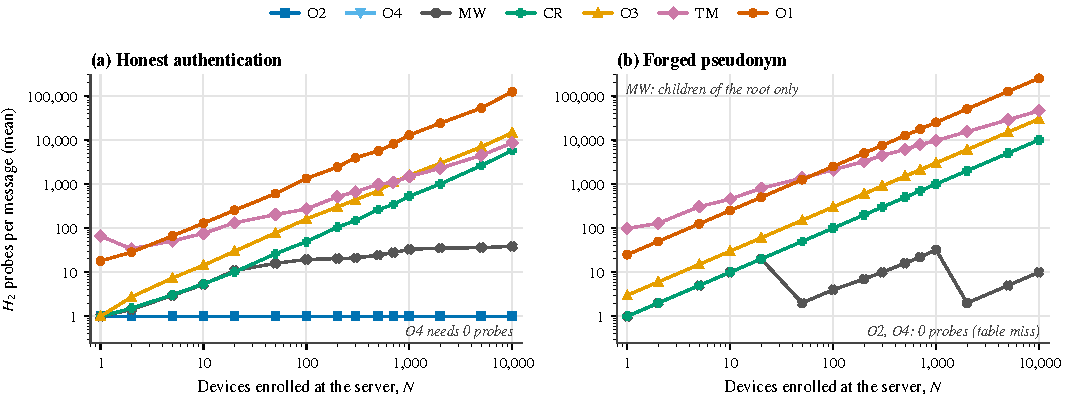
\includegraphics[width=\textwidth]{figures/fig_probes.pdf}
\caption{Probes per message at one server, measured on the implementation (log--log): (a) honest authentication, (b) a forged, random pseudonym}
\label{fig:probes}
\end{figure}

\subsection*{Session latency and storage in the network model}
Table~\ref{tab:ranked} ranks the strategies by mean session latency at $N=1000$ with 5\% adversaries, from the 960 OMNeT++ runs; their closed-form costs are given in Table~\ref{tab:design}. The \emph{base} column ($N=1$) is the value published in~\cite{base}: 23.68\,ms (Tables~III and~V) and 320 bits (Table~VI). Storage is Table~VI's 320 bits per enrolled device plus the resolution state, averaged over the servers. Figures~\ref{fig:latency} and~\ref{fig:storage} plot the same data.

\begin{table}[H]
\centering
\caption{Strategies ranked by mean session latency at $N=1000$ (5\% adversaries); mean of five seeds}
\label{tab:ranked}
\scriptsize
\setlength{\tabcolsep}{3pt}
\renewcommand{\arraystretch}{1.2}
\begin{tabular}{|c|l|r|r|r|r|r||r|r|r|r|r|}
\hline
 & & \multicolumn{5}{c||}{\textbf{Mean session latency (ms)}} & \multicolumn{5}{c|}{\textbf{Storage per server (KB)}}\\ \hline
\textbf{\#} & \textbf{Strategy} & base & 10 & 100 & 500 & 1000 & base & 10 & 100 & 500 & 1000\\ \hline
1 & O2 Counter + precomputed table & 23.68 & 24.17 & 24.25 & 24.40 & 24.40 & 0.04 & 0.93 & 8.78 & 46.1 & 92.9\\ \hline
2 & O4 Clock + per-epoch table & 23.68 & 23.85 & 23.93 & 24.22 & 24.59 & 0.04 & 0.47 & 4.39 & 23.1 & 46.4\\ \hline
3 & MW Key tree & 23.68 & 24.44 & 27.96 & 30.86 & 31.38 & 0.04 & 0.10 & 0.97 & 5.16 & 10.4\\ \hline
4 & CR Randomized hash lock & 23.68 & 24.44 & 28.86 & 51.71 & 94.89 & 0.04 & 0.10 & 0.95 & 5.02 & 10.1\\ \hline
5 & O3 Clock + linear scan & 23.68 & 24.94 & 38.99 & 176.1 & 1,108 & 0.04 & 0.16 & 1.53 & 8.03 & 16.1\\ \hline
6 & TM Rainbow time--memory trade-off & 23.68 & 38.33 & 516.5 & 5,228 & 12,850 & 0.04 & 2.26 & 10.8 & 36.5 & 59.9\\ \hline
7 & O1 Counter + linear scan & 23.68 & 36.02 & 507.9 & 16,947 & 44,010 & 0.04 & 0.12 & 1.15 & 6.02 & 12.1\\ \hline
\end{tabular}
\end{table}

\begin{figure}[H]
\centering
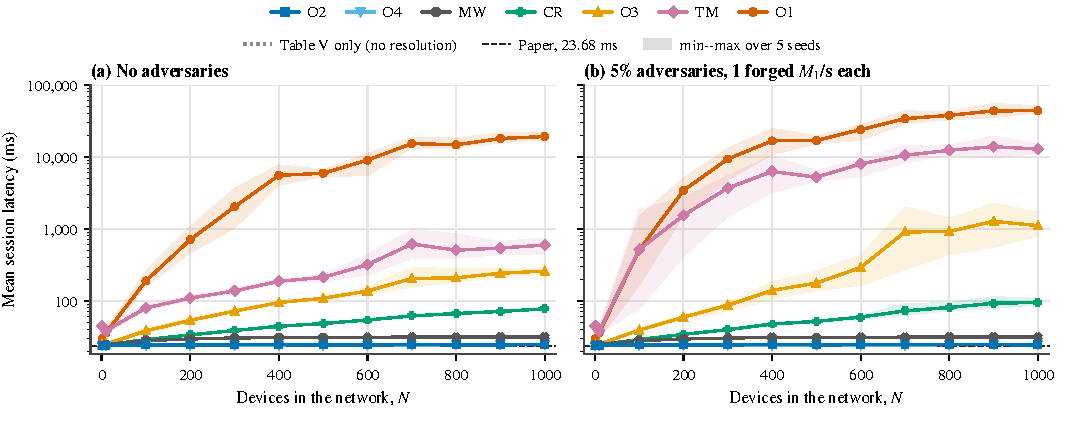
\includegraphics[width=\textwidth]{figures/fig_latency.pdf}
\caption{Mean session latency against network size in the OMNeT++ model (log scale; band: minimum to maximum over five seeds). Dotted: the paper's cost model with no resolution. Dashed: the paper's 23.68\,ms. (a) No adversaries, (b) 5\% adversaries}
\label{fig:latency}
\end{figure}

\begin{figure}[H]
\centering
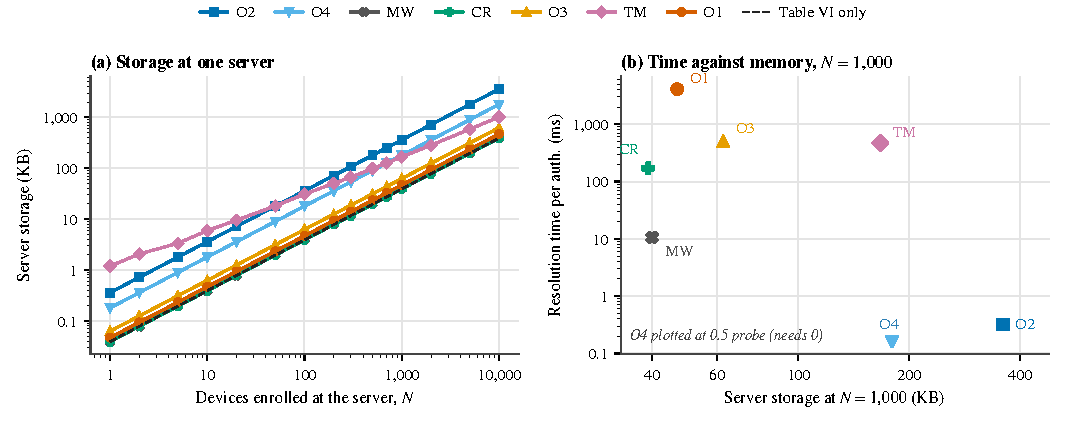
\includegraphics[width=\textwidth]{figures/fig_storage.pdf}
\caption{(a) Server storage at one server (Table~VI's 320 bits per device plus the resolution state); (b) resolution time per authentication ($T_H=0.32$\,ms per probe) against storage at $N=1000$}
\label{fig:storage}
\end{figure}

\subsection*{Desynchronisation}
Table~\ref{tab:desync} is the output of \texttt{desync\_check.py} for counter epochs (re-run for this report; identical to the committed output). An adversary drops $k$ consecutive $M_1$ messages, and the next three honest handshakes are attempted.

\begin{table}[H]
\centering
\caption{Next three honest handshakes after $k$ dropped $M_1$ messages (counter epochs, $F=8$)}
\label{tab:desync}
\small
\begin{tabular}{|c|c|l|}
\hline
\textbf{Dropped $k$} & \textbf{Earlier successful session} & \textbf{Next three honest handshakes}\\ \hline
6 & no / yes & ok, ok, ok\\ \hline
7 & no / yes & ok, ok, ok\\ \hline
8 & no / yes & UnknownPeerError (all three)\\ \hline
9 & no / yes & UnknownPeerError (all three)\\ \hline
12 & no / yes & UnknownPeerError (all three)\\ \hline
\multicolumn{3}{|l|}{Device restart after three successful handshakes (epoch kept in RAM): ReplayDetected}\\ \hline
\end{tabular}
\end{table}

\subsection*{Sensitivity to the assumptions}
The base paper does not fix the adversary share and rate, the authentication window or the enrolment rule, and the per-probe cost $T_H=0.32$\,ms is the paper's constant rather than a measurement on our hardware. Their effect was examined in two ways, without new simulation runs (\texttt{evaluation/resolution/sensitivity.py}, output in \texttt{sensitivity.txt}).

First, the committed OMNeT++ sweep already contains every strategy with and without adversaries (Table~\ref{tab:advcmp}). At $N=1000$ the ranking is identical in both cases.

\begin{table}[H]
\centering
\caption{Simulated mean session latency at $N=1000$ with and without adversaries (ms, mean of five seeds)}
\label{tab:advcmp}
\small
\begin{tabular}{|l|r|r|r|r|r|r|r|}
\hline
 & \textbf{O2} & \textbf{O4} & \textbf{MW} & \textbf{CR} & \textbf{O3} & \textbf{TM} & \textbf{O1}\\ \hline
No adversaries & 24.43 & 24.48 & 31.43 & 77.18 & 258.7 & 595.8 & 19,219\\ \hline
5\% adversaries & 24.40 & 24.59 & 31.38 & 94.89 & 1,108 & 12,850 & 44,010\\ \hline
\end{tabular}
\end{table}

Second, the offered load $\rho$ of the mean server at $N=1000$ was computed from the committed cost model and runs as $\rho=\lambda_h(S+h(n)\,T_H)+\lambda_a f(n)\,T_H$, where $S=11.84$\,ms is the paper's server cost per session, $h$ and $f$ are the measured honest and forged probes, $n=258$ is the mean number of devices enrolled per server, and $\lambda_h$ and $\lambda_a$ are the honest and forged request rates per server (O4 adds its per-epoch extension). A server with $\rho\ge1$ cannot keep up and its queue grows for the whole window. Table~\ref{tab:sens} varies one assumption at a time from the baseline.

\begin{table}[H]
\centering
\caption{Offered load $\rho$ of the mean server at $N=1000$, one assumption varied at a time (baseline: 5\% adversaries at 1\,Hz, 10\,s window, reachable enrolment, $T_H=0.32$\,ms; $\rho\ge1$ means saturated)}
\label{tab:sens}
\small
\begin{tabular}{|l|r|r|r|r|r|r|r|}
\hline
\textbf{Case} & \textbf{O2} & \textbf{O4} & \textbf{MW} & \textbf{CR} & \textbf{O3} & \textbf{TM} & \textbf{O1}\\ \hline
Baseline & 0.02 & 0.03 & 0.04 & 0.19 & 0.52 & 1.68 & 4.16\\ \hline
No adversaries & 0.02 & 0.03 & 0.04 & 0.11 & 0.27 & 0.41 & 2.09\\ \hline
20\% adversaries & 0.02 & 0.03 & 0.05 & 0.44 & 1.26 & 5.47 & 10.3\\ \hline
Adversary rate 2\,Hz & 0.02 & 0.03 & 0.04 & 0.27 & 0.77 & 2.94 & 6.22\\ \hline
Window 5\,s & 0.05 & 0.06 & 0.08 & 0.30 & 0.79 & 2.09 & 6.25\\ \hline
Window 20\,s & 0.01 & 0.02 & 0.02 & 0.14 & 0.38 & 1.47 & 3.11\\ \hline
$T_H=0.16$\,ms & 0.02 & 0.03 & 0.03 & 0.11 & 0.27 & 0.85 & 2.09\\ \hline
$T_H=0.64$\,ms & 0.03 & 0.04 & 0.06 & 0.36 & 1.01 & 3.33 & 8.29\\ \hline
Nearest enrolment & 0.02 & 0.02 & 0.04 & 0.04 & 0.06 & 0.36 & 0.35\\ \hline
\end{tabular}
\end{table}

\subsection*{Formal verification}
Table~\ref{tab:fv} lists the ProVerif~2.05 results (committed logs in \path{evaluation/formal_verification/logs/}); every model finishes in under one second.

\begin{table}[H]
\centering
\caption{ProVerif results}
\label{tab:fv}
\small
\renewcommand{\arraystretch}{1.15}
\begin{tabularx}{\textwidth}{|l|X|l|}
\hline
\textbf{\#} & \textbf{Property} & \textbf{Result}\\ \hline
Q1 & Session key secret (device side), honest pair & true\\ \hline
Q2 & Session key secret (server side), honest device & true\\ \hline
Q3 & Server accepts $M_1$ of honest $V$ $\Rightarrow$ $V$ sent it (non-injective agreement on $V,R,N_i,t$) & true\\ \hline
Q4 & Same, injective (no replay state in the model) & false (replay trace)\\ \hline
Q5 & Device accepts $M_2$ $\Rightarrow$ server derived the same key with the same nonces (injective) & true\\ \hline
FS & Session key secret after a later leak of $k^\star$ & false\\ \hline
U1 & Unlinkability, counter epochs (observational equivalence) & true\\ \hline
U2 & Unlinkability, clock epochs, two sessions in one epoch & fails (equal PIDs)\\ \hline
\end{tabularx}
\end{table}

\section{Result Analysis}
\textbf{Ranking.} The two table strategies, O2 and O4, stay within 1\,ms of the paper's 23.68\,ms up to 1,000 devices (24.40\,ms and 24.59\,ms). O2 needs one probe to slide its window and O4 only its per-epoch extension. Their cost is memory: at 1,000 devices about 93\,KB and 46\,KB per server, against 10\,KB for Table~VI alone. The key tree (MW) is third at 31.4\,ms, but it changes $M_1$, and a compromised device leaks the internal keys it shares with others. The randomized hash lock (CR) needs no extra state, but its latency grows linearly, to 95\,ms. The three scanning strategies over epochs saturate the server: clock scan (O3) at 1.1\,s, the time--memory trade-off at 12.9\,s, and the counter scan (O1) at 44\,s. For O1 and TM, the spread across seeds at $N=1000$ is 10.6\,s and 4.5\,s, because latency depends on how many devices and adversaries share the busiest server.

\textbf{Honest load against forged load.} Without adversaries (Figure~\ref{fig:latency}a), O1 already reaches 19.2\,s at 1,000 devices. Each honest authentication costs about $12.5\,n$ probes, which is 1.0\,s of hashing at the $n\approx258$ devices that a server enrols at $N=1000$, and arrivals outpace this, so the server queue grows. Forged load (Figure~\ref{fig:latency}b) roughly doubles the latency, because every forged pseudonym costs a full miss scan of $Wn$ probes. Such a pseudonym never resolves to a device, so the block-list, which counts failures per device, never sees it. At one server (Figure~\ref{fig:probes}b), a forgery at $n=10{,}000$ costs O1 250,000 probes and TM about 46,000, but costs O2 and O4 nothing, because a table miss needs no hash.

\textbf{Time against memory.} No strategy that keeps the wire format is both fast and small (Figure~\ref{fig:storage}b). O2 buys constant time with $F$ table entries per device (328\,KB in total at $n=1000$), and O4 with $W_t$ entries per device (144\,KB). TM sits in between, at 131\,KB and 1,478 probes, and is dominated here because its table must cover a device's whole lifetime ($m=128$ epochs), not only the current window. MW is the only point that is both small and fast, and it pays with a different $M_1$ and a weaker privacy model.

\textbf{Desynchronisation.} With counter epochs the device advances $t$ every time it builds $M_1$, and the server searches at most $F$ epochs ahead of the last one it accepted. An adversary who drops $F$ consecutive $M_1$ messages therefore locks the device out for good (Table~\ref{tab:desync}, with $F=8$), with or without an earlier successful session. The threshold is the window parameter $F$, which the specification does not fix; a larger $F$ delays the lockout but does not remove it. The lockout holds for O1 and O2, and a unit test checks it for both. A device whose counter lives in RAM is also rejected as a replay after a restart. Message dropping is within the threat model of~\cite{base}. Clock epochs (O3, O4), CR and MW have no per-device counter and cannot desynchronise this way; TM tolerates any number of drops until $t$ reaches the lifetime $m$.

\textbf{Security properties.} The ProVerif results separate the properties that the resolver cannot affect from those it decides. Session-key secrecy (Q1, Q2), agreement on $(V,R,N_i,t)$ (Q3) and injective key agreement for the device (Q5) hold for every correct resolver; Q5 holds because $N_i$ is fresh and bound as associated data of $M_2$. Injective authentication of the device (Q4) fails without replay state: ProVerif finds a trace in which one $M_1$ is accepted twice, so injectivity rests on the epoch window (O1, O2, TM) or the nonce cache (O3, O4), which the specification leaves open. With clock epochs the attacker links two sessions in one epoch by testing their pseudonyms for equality (U2); with counter epochs the equivalence holds (U1). Forward secrecy does not hold, and the base paper does not claim it: a later leak of $k^\star$ reveals $N_i$, $N_j$ and $t$ from the ciphertexts and with them the session key.

\textbf{Sensitivity to the assumptions.} The adversaries change the absolute latencies but not the ranking: without them O1 still reaches 19.2\,s, and O2, O4 and MW move by less than 0.2\,ms (Table~\ref{tab:advcmp}). Across adversary shares of 0 to 20\%, adversary rates of 0.5 to 2\,Hz, windows of 5 to 20\,s and $T_H$ from 0.16 to 0.64\,ms, the order of the strategies by offered load is the order of Table~\ref{tab:ranked}, and O2 and O4 stay below $\rho=0.06$ (Table~\ref{tab:sens}). The absolute figures do depend on the assumptions: O1 saturates the mean server unless $T_H<0.076$\,ms, and with 20\% adversaries or $T_H=0.64$\,ms O3 saturates as well. $\rho$ describes the mean server; the busiest server enrols up to 396 devices, which is why O3 already queues in the simulation at $\rho=0.52$. The enrolment rule matters most. If a server enrols only the devices attached to it ($n\approx20$), no strategy saturates, and CR and MW swap places, as do TM and O1, but O2 and O4 remain first. The window parameters $L$, $F$ and $W_t$ act only through the closed forms of Table~\ref{tab:design}: the lockout threshold equals $F$, and O2's state grows as $40F+8$ bytes per device. The recommendation to precompute therefore holds under every assumption varied, whereas figures such as the 44\,s of O1 hold only under the baseline.

\textbf{What the validation shows and does not show.} Every result rests on a check that can be rerun: the reference vectors and the interoperability run for the implementations, the closed forms for the probe counts, the model without resolution against the paper's 23.68\,ms (23.86\,ms at $N=1$ and 24.07\,ms at $N=1000$, a 0.8 to 1.7\% difference from airtime and quantisation), and ProVerif for the security properties. The offered-load analysis, computed independently of the simulator, also orders the strategies exactly as the simulation does. The checks have limits. The authors' code is not available, so the vectors encode our reading of Section~III of~\cite{base}: they show that both implementations agree with that reading, not that it is the authors' intent. The network model is checked against the paper only where the paper gives a figure, at one device and with no resolution, and its behaviour in saturation has not been compared with another simulator.

\textbf{Comparison with the objectives.} Table~\ref{tab:objectives} relates each objective of Section~1.3 to the evidence obtained.

\begin{table}[H]
\centering
\caption{Objectives and the evidence obtained}
\label{tab:objectives}
\small
\renewcommand{\arraystretch}{1.2}
\begin{tabularx}{\textwidth}{|c|>{\raggedright\arraybackslash}p{0.33\textwidth}|X|}
\hline
\textbf{\#} & \textbf{Objective} & \textbf{Evidence}\\ \hline
1 & Conformant Python and C implementations & 15/15 vector checks in each; 5/5 interoperable handshakes; 125 tests pass\\ \hline
2 & Resolution required; open choices identified & Five-step argument from the specification and the vectors (Section~3.3); two open choices\\ \hline
3 & Seven strategies, measured and validated & Closed forms exact for O1--O4 and CR; honest means within 4 SE; MW within its bound; TM 9 misses in 2,100\\ \hline
4 & Network pricing and ranking & 960 OMNeT++ runs; O2 at 24.4\,ms and O1 at 44\,s at $N=1000$ with 5\% adversaries; ranking unchanged without adversaries and under every assumption varied (Table~\ref{tab:sens})\\ \hline
5 & Failure modes & Forged pseudonyms cost O1 $Wn$ probes and O2/O4 none; lockout after $F$ dropped messages ($F=8$ here)\\ \hline
6 & Formal analysis & Q1--Q3, Q5, U1 true; Q4, FS false; U2 fails\\ \hline
7 & Open release & Code, models, data and logs in the public repository\\ \hline
\end{tabularx}
\end{table}

\section{Limitations}
\begin{itemize}
\item The network model is our model of the paper's stated environment, not the authors' simulation, which is not available. The adversary share and rate, the 10\,s authentication window and the enrolment rule are our assumptions, and the saturated latencies of O1, O3 and TM depend on them.
\item Probes are priced with the paper's constant $T_H=0.32$\,ms; no hardware timings are reported.
\item CR and MW change $M_1$ and are modelled at the resolution level only, not in the full handshake.
\item The TM parameters (six tables, $m=128$) are one point on its trade-off curve, and TM measurements vary between runs because peer secrets are drawn from operating-system randomness.
\item The epoch, window and table parameters are our choices, not the paper's; conformance means agreement with our reading of Section~III.
\item The Python key store is demonstration-grade, re-keying (Eq.~24) is a stub, and coverage (Eqs.~10, 23) is an abstract predicate with no radio model.
\end{itemize}

\section{Observation/Remarks}
\begin{itemize}
\item \textbf{The original implementation was the worst case.} Our first server, written before the resolution study, resolved pseudonyms with a linear scan over a counter window, which is strategy O1. Nothing in the paper warned against it, and it turned out to be the slowest strategy and the one most exposed to forged traffic.
\item \textbf{A precomputed table removes both the scaling and the denial-of-service problem.} Because a table miss needs no hash, forged pseudonyms become free for the server to reject, at a cost of about $40F$ bytes per device.
\item \textbf{The block-list does not protect resolution.} It counts failures per device, but a forged pseudonym never resolves to a device, so the expensive work happens before the block-list can act.
\item \textbf{Specification ambiguities.} Section~II and Section~III of the paper describe different online phases; the implementation follows Section~III, the version covered by the paper's security sketch. The paper also leaves open whether $\mu_1$ covers the clear pseudonym and how $\sigma_2$ is built; these choices are recorded in the assumption register.
\item \textbf{Reproducibility of the measurements.} Re-running the probe sweep for this report reproduced every non-TM row of \texttt{measured.csv} exactly. The TM rows differ, as the repository documents: in our re-run the honest probes per $S^{2/3}$ ranged from 0.42 to 0.67 (0.50 to 0.73 in the committed run) and 7 of 2,100 pseudonyms were missed (9 in the committed run). Regenerating the figures and the ranked table from the committed data reproduced them exactly.
\item \textbf{Independent vectors were essential.} Generating the vectors with code that shares nothing with either implementation fixed the message layout on which the whole gap argument relies, and made the C port's conformance checkable in CI without hardware.
\end{itemize}

\section{Conclusion}
The protocol of~\cite{base} was implemented in Python and, on the device side, in C, and both reproduce the independent reference vectors byte for byte. Seven resolution strategies were implemented and measured, and their probe counts match the closed forms. Under the paper's own constants and network, the choice of resolver decides whether the server stays at the paper's 23.68\,ms per session or saturates at tens of seconds: O2 holds 24.4\,ms at 1,000 devices with 5\% adversaries, while O1 reaches 44\,s. The choice also decides whether forged pseudonyms are free to send and whether $F$ dropped messages ($F=8$ here) lock a device out. Varying the assumptions changes these absolute figures but not the ranking. The formal analysis shows that secrecy and agreement do not depend on the choice, while unlinkability and injective authentication do. All seven objectives were met, within the limitations listed above. The next chapter concludes the report and outlines future work.
